\documentclass[convert={density=900,size=1080x800,outext=.png}]{standalone}
\usepackage{tikz}
\usetikzlibrary{calc, positioning}
\usetikzlibrary{arrows.meta}
\usetikzlibrary{matrix}
\usetikzlibrary{shadows}
\usepgflibrary{shapes.misc}
\usepgflibrary{{shapes.geometric}}
\usetikzlibrary{arrows,positioning,shapes}

\pgfdeclarelayer{shadow} 
\pgfsetlayers{shadow,main}
\def\shadowradius{3pt}


\def\lw{2mm}        % Arrow line width
\def\mw{2cm}        % Minimum width of component
\def\mh{1.75cm}     % Minimum height of component
\def\trianglecoordinate{2mm}    % Starting coordinate clock input triangle of components

\newcommand\drawshadowbis[1]{
    \begin{pgfonlayer}{shadow}
        \fill[inner color=black,outer color=white] ($(#1.south west)$) circle (\shadowradius);
        \fill[inner color=black ,outer color=white] ($(#1.north west)$) circle (\shadowradius);
        \fill[inner color=black ,outer color=white] ($(#1.south east)$) circle (\shadowradius);
        \fill[inner color=black,outer color=white] ($(#1.north east)$) circle (\shadowradius);
        \fill[ top color=black, bottom color=white] ($(#1.south west)+((0,-\shadowradius)$) rectangle ($(#1.south east)$);
        \fill[left color=black,right color=white] ($(#1.south east)$) rectangle ($(#1.north east)+((\shadowradius,0)$);
        \fill[bottom color=black,top color=white] ($(#1.north west)$) rectangle ($(#1.north east)+((0,\shadowradius)$);
        \fill[right color=black,left color=white] ($(#1.south west)$) rectangle ($(#1.north west)+(-\shadowradius,0)$);
    \end{pgfonlayer}
    }

\tikzset{
    border/.style = { 
        draw, rectangle, minimum width=1.5cm, minimum height=1cm, ultra thick
    },
    pics/Component/.style n args = {2}{
        code = {
            \node [border, align=center](-edge){#1};
            \draw[thick] ([xshift=\trianglecoordinate] -edge.south) -- ([yshift=\trianglecoordinate] -edge.south);
            \draw[thick] ([xshift=-\trianglecoordinate] -edge.south) -- ([yshift=\trianglecoordinate] -edge.south);
            \draw[thick] (-edge.south) |- ++(-3mm, -4mm) node[xshift=-2mm, yshift=-1mm] {#2}; 
    }}
    }

\tikzset{
    clockborder/.style = { 
        trapezium, trapezium angle=60, minimum width=1cm, draw, very thick
    },
    Clock/.pic = {
        \node [clockborder, shape border rotate=-180](-clockedge){#1};
        \draw[very thick] (-clockedge.east) -- ++(2cm, 0cm);
        \def\sft{0.5}
        \foreach \x in {0, 0.5, 1, 1.5}{
            \draw[very thick] (\x + \sft, 0.1) -| ++(0.25cm, 0.25cm) -| ++ (0.25cm, -0.25cm);
        }
    },
}

\begin{document}
    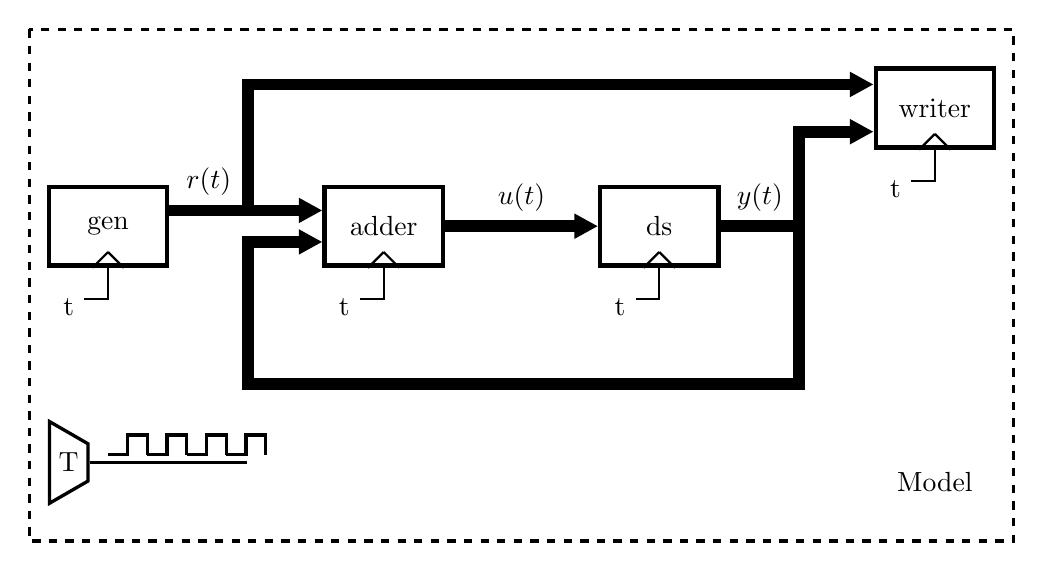
\begin{tikzpicture}[every node/.style={font=\normalsize}]
        % Place the blocks 
        \draw(-3.5, 0) pic (gen) {Component={gen}{t}};
        \draw pic (adder) {Component={adder}{t}};
        \draw(3.5, 0) pic (ds) {Component={ds}{t}};
        \draw(7, 1.5) pic (writer) {Component={writer}{t}};
        \begin{scope}[line width=1.5mm, ->, >={Triangle[width=3mm,length=3mm]}]
            \draw[-] ([yshift=2mm] gen-edge.east) -- ++(1cm, 0cm) node[midway, anchor=south]{$r(t)$} coordinate(d); 
            \draw (d) -- ([yshift=2mm]  adder-edge.west);
            \draw (adder-edge.east) -- node[midway, anchor=south]{$u(t)$} (ds-edge.west);
            \draw[-] (ds-edge.east) -- ++(1cm, 0cm) node[midway, anchor=south]{$y(t)$} coordinate (a);
            \draw (a) |- ([yshift=-3mm] writer-edge.west);
            \draw[-] (a) |- ++(-7cm, -2cm) coordinate (c);
            \draw ([yshift=-0.75mm]c) |- ([yshift=-2mm] adder-edge.west);
            \draw[-] ([yshift=2mm] gen-edge.east) -- ++ (1cm, 0cm) coordinate(d);
            \draw (d) |- ([yshift=3mm] writer-edge.west);
        \end{scope}
        \draw[very thick, dashed] (-4.5, 2.5) rectangle (8, -4);
        \node at (7, -3.25) {Model};

         % \Place clock 
        \begin{scope}[shift={(-4cm, -3cm)}]
            \draw pic(clk) {Clock={T}} ;
        \end{scope}

    \end{tikzpicture}
\end{document}
